\begin{figure}
\centering

\ifpdf
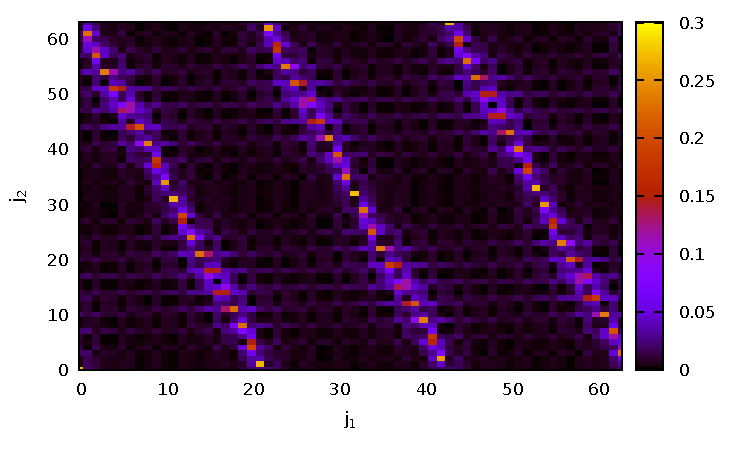
\includegraphics[angle=0]
{./part4/quantcomp/picdiscretlog4.pdf}
\else
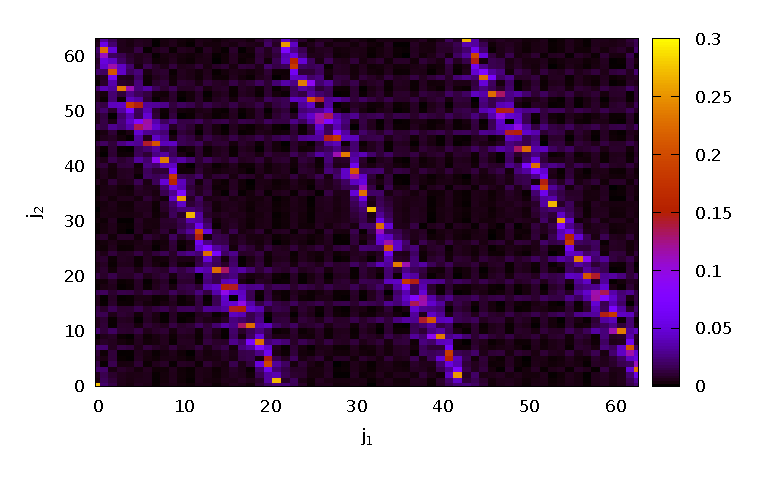
\includegraphics[angle=0]
{./part4/quantcomp/picdiscretlog4.eps}
\fi

%\input ./part4/quantcomp/picdiscretlog2.tex

\caption{Fourier transform of the samples of the function 
$f'(x_1, x_2)$
Number of samples $M=64$. The three lower maxima have coordinates $\approx (20,1), (41,2.2), (62,
3)$, giving the following estimates for $x$: $x \approx 20, 18.6, 20.6$,
which is close to the real value $x = 19$
} 
\label{fig:part4:quantcomp:dl4}
\end{figure}